    % Chapter AddressFamily

\chapter{AF\_APNA} % Main chapter title

\label{address_family}

\section{Background}
\subsection{What is an address family?}
The address family parameter (address\_family) on a \texttt{BSD} socket() API determines the format of the address structure to be used on socket APIs.

Address family protocols provide the network transportation of application data from one application to another (or from one process to another within the same system). The application specifies the network transport provider on the protocol parameter of the socket. For example the most popular address are following:
\begin{itemize}
    \item \textbf{AF\_INET address family} \\
    This address family provides interprocess communication between processes that run on the same system or on different systems.
    \item \textbf{AF\_INET6 address family} \\
    This address family provides support for the Internet Protocol version 6 (IPv6). AF\_INET6 address family uses a 128 bit (16 byte) address.
    \item \textbf{AF\_UNIX address family} \\
    This address family provides interprocess communication on the same system that uses the socket APIs. The address is actually a path name to an entry in the file system.
\end{itemize}

\section{APNA Address Family}
\subsection{Why do we need a new address family?}
In the approach presented in Chapter \ref{apna_overlay} there was one major drawback that it was wasting around 8-32 bytes depending upon whether endhost were using IPv4 or IPv6 address for communication. Conceptually speaking it was more of an hack rather than a well integrated solution inside SCION. 

Those bytes could be better utilized if we can introduce a new address family for APNA address. Instead of wasting space with random IPv4/IPv6 addresses use EphIDs as source and destination address. This would result in higher MTU for data packets as they don't have encapsulate EphIDs inside it and in the end would result in saving of lots of bytes which are better utilized by using EphIDs.

\subsection{Characteristics of APNA Address Family}
\subsubsection{AF\_APNA address family}
This address family provides support for APNA protocol. AF\_APNA uses a 128 bit (16 bytes) Ephemeral IDs as address. Looking at the address size it looks very similar to IPv6 addresses but they have very different meaning. APNA address representation would be grouped as follows:
\begin{center}
deadcafe:baadf00ddeadbeef:40044b1d
\end{center}
First 4 bytes represents the initialization vector that was used to encrypt the host id. Next 8 bytes represents the encrypted host id. Last 4 bytes represents the MAC over first 12 bytes. Representation is not user friendly but it does not matter as users would never be using those addresses like IPv4/IPv6 addresses as these are Ephemeral address and exists only for a short duration. Its representation is like that mainly for the debugging reason it makes it easy to identify what went wrong while generating EphIDs.

\section{Communication Overview}
\begin{figure}[th!!]
\centering
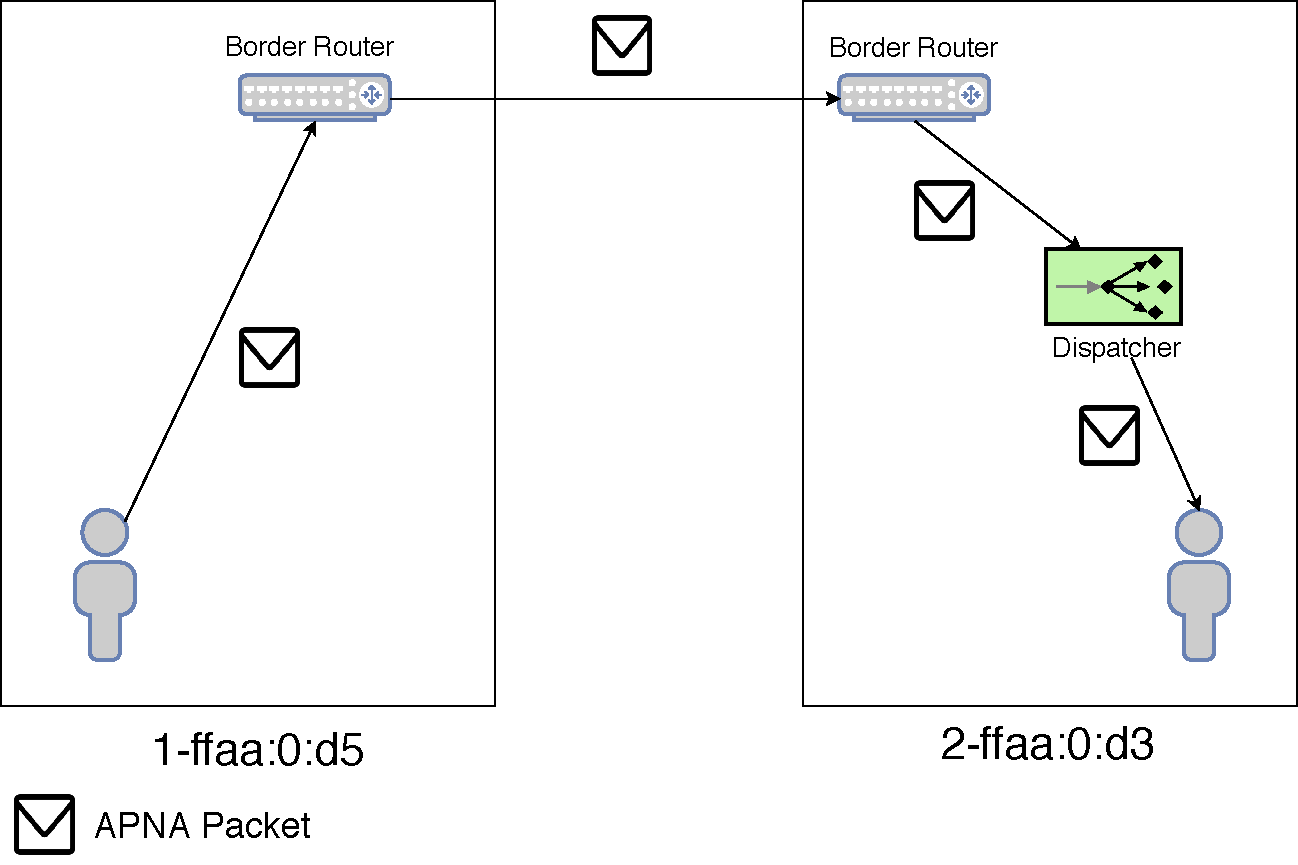
\includegraphics[scale=0.5]{Figures/address_family_comm.pdf}
\decoRule
\caption[APNA Service Incoming Packet]{Communication overview using APNA address family}
\label{fig:apna_address_comm}
\end{figure}
Fig \ref{fig:apna_address_comm} represents a scenario in which host in ISD 1 and AS \texttt{ffaa:0::d5} wants to communicate with another host in ISD 2 and AS \texttt{ffaa:0::d3}. In order to do so sender first needs to resolve the path to the receiver using SCIOND. Once it obtains the path it will forward the packet to the first hop border router. After that border router will forward the path to destination border router depending upon the path chosen by the sender.

Last hop border router needs to parse the packet to find out which dispatcher it needs to forward the packet and the dispatcher would eventually forward it to the right host. In order to obtain IP address from EphID border router uses the algorithm described in Sec \ref{algo:addr_fam_comm} and it uses the fixed \texttt{EndHostPort(30041)} to forward it to dispatcher. Dispatcher also performs the similar translation to find the IP address of host it needs to forward it to. It gets the port number which it has stored in a hashmap when the host registered with the dispatcher while starting the service.

\subsection{Algorithm to obtain IP address from EphID} \label{algo:addr_fam_comm}
\begin{algorithmic}
 \STATE $P \leftarrow $ Parse the SCION Packet
 \STATE $DstEphID  \leftarrow P.L4Header.DstEphID $ 
\end{algorithmic}
  
\begin{algorithmic}
 \IF{$DstEphID$ is not nil}
 \STATE $HID \leftarrow Decrypt(DstEphID)$
 \IF{$HID$ is not nil}
 \STATE $IP \leftarrow GetIPFromHID(HID)$
 \ELSE
 \STATE Drop the packet and abort; 
 \ENDIF
 \ELSE
 \STATE Drop the packet and abort;
 \ENDIF
\end{algorithmic}

\section{Modifications required in the current infrastructure}
\subsection{SCION-APNA Packet Structure}
\begin{figure}[th!!]
\centering
\noindent
\makebox[\textwidth]{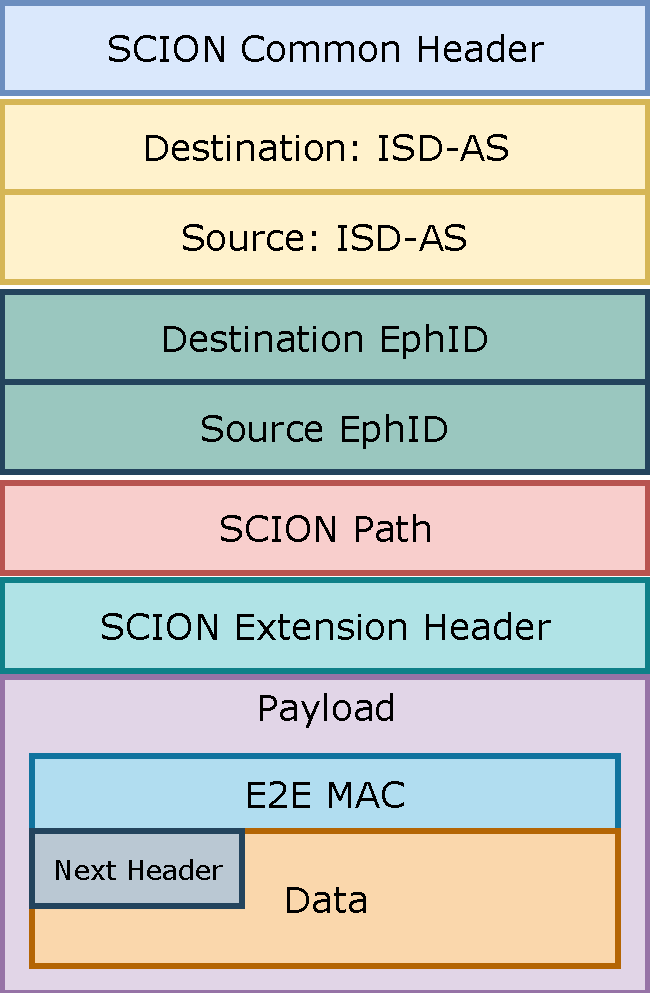
\includegraphics[scale=0.6]{Figures/apna_af.pdf}}
\decoRule
\caption[APNA packet structure using its own address family]{APNA Packet structure  using its own address family}
\label{fig:apna_scion_pkt}
\end{figure}

\subsection{Border Router}
\subsection{Dispatcher}
\subsection{Address Types}
\texttt{HostAddrType} enum needs to be extended with new \texttt{HostTypeAPNA} (4) for both Golang and Python side. As a matter of fact C's packet parsing logic required by dispatcher also needs to be modified to correctly parse this new address family.
